
\definecolor{cb3b3b3}{RGB}{179,179,179}


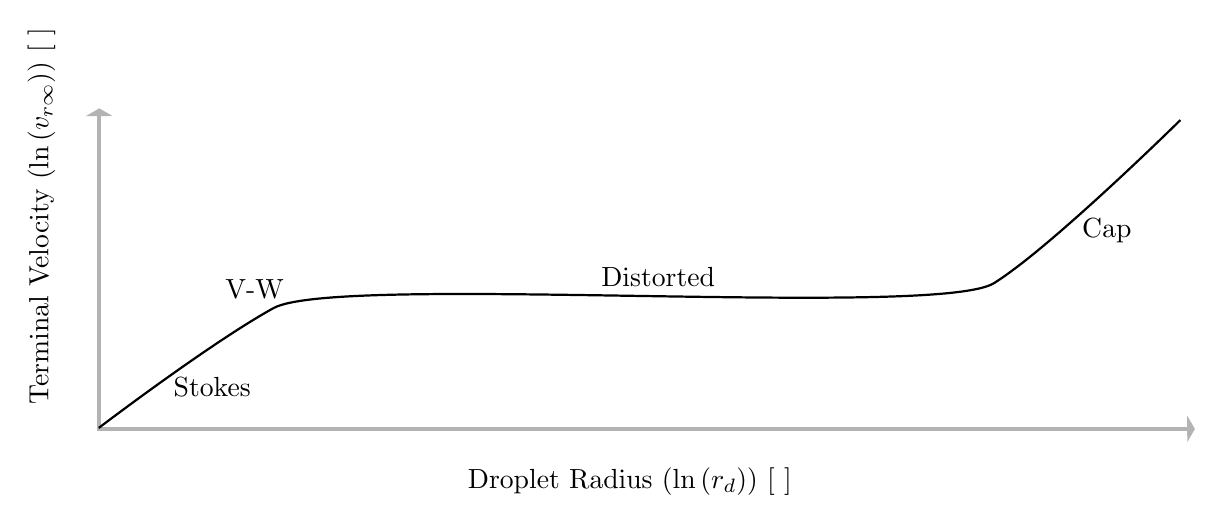
\begin{tikzpicture}[y=0.80pt, x=0.8pt,yscale=-1, inner sep=0pt, outer sep=0pt]
\begin{scope}[shift={(0,-872.35975)}]
  \path[fill=cb3b3b3] (533.6587,1012.9418) -- (537.1719,1019.0269) --
    (533.7256,1024.9960) -- cycle;
  \path[draw=cb3b3b3,line join=miter,line cap=butt,miter limit=4.00,line
    width=1.600pt] (42.2394,877.1861) -- (42.2394,1018.9689) --
    (534.6470,1018.9689);
  \path[fill=cb3b3b3] (36.2123,877.7175) -- (42.2974,874.2043) --
    (48.2665,877.6506) -- cycle;
  \path[fill=black] (208.80496,1049.1238) node[above right] (text3075-4-1-2-9-9-5)
    {Droplet Radius ($\ln \left( r_{d} \right)$) [ ]};
  \begin{scope}[shift={(0,774.35975)},fill=black]
  \end{scope}
  \path[cm={{0.0,-1.0,1.0,0.0,(0.0,0.0)}},fill=black] (-1007.9703,9.9532785)
    node[above right] (text3035) {\rotatebox{90}{Terminal Velocity ($\ln \left(
    v_{r\infty} \right)$) [ ]}};
  \path[shift={(0,872.35975)},fill=black] (22.864506,15.972022) node[above right]
    (text3821) {};
  \path[shift={(0,872.35975)},draw=black,line join=miter,line cap=butt,line
    width=0.800pt] (42.0877,146.1795) .. controls (42.0877,146.1795) and
    (92.3891,107.8615) .. (121.0021,92.0668) .. controls (149.6150,76.2721) and
    (420.6043,96.9184) .. (446.4301,80.7933) .. controls (472.2558,64.6682) and
    (530.6054,7.1399) .. (530.6054,7.1399);
  \path[shift={(0,872.35975)},fill=black] (75.908142,131.8998) node[above right]
    (text4860) {Stokes};
  \path[fill=black] (99.206673,959.91718) node[above right] (text4864) {V-W};
  \path[fill=black] (269.06055,954.65619) node[above right] (text4868)
    {Distorted};
  \path[fill=black] (486.26303,935.11548) node[above right] (text4872) {Cap};
\end{scope}

\end{tikzpicture}
